\documentclass{beamer}

\usepackage{Haust2016glærur}

\title{Stærðfræðimynstur í tölvunarfræði}
\subtitle{Vika 13, seinni fyrirlestur}

\begin{document}

\begin{frame}
\titlepage
\end{frame}


\section{Inngangur}

\begin{frame}{Í síðasta tíma}
\begin{itemize}
 \item Spanntré
 \item Dýptarleit og breiddarleit
 \item Léttustu spanntré
 \begin{itemize}
  \item Reiknirit Prims og Kruskals
 \end{itemize}
\end{itemize}
\end{frame}

\begin{frame}{Reiknirit Prims}
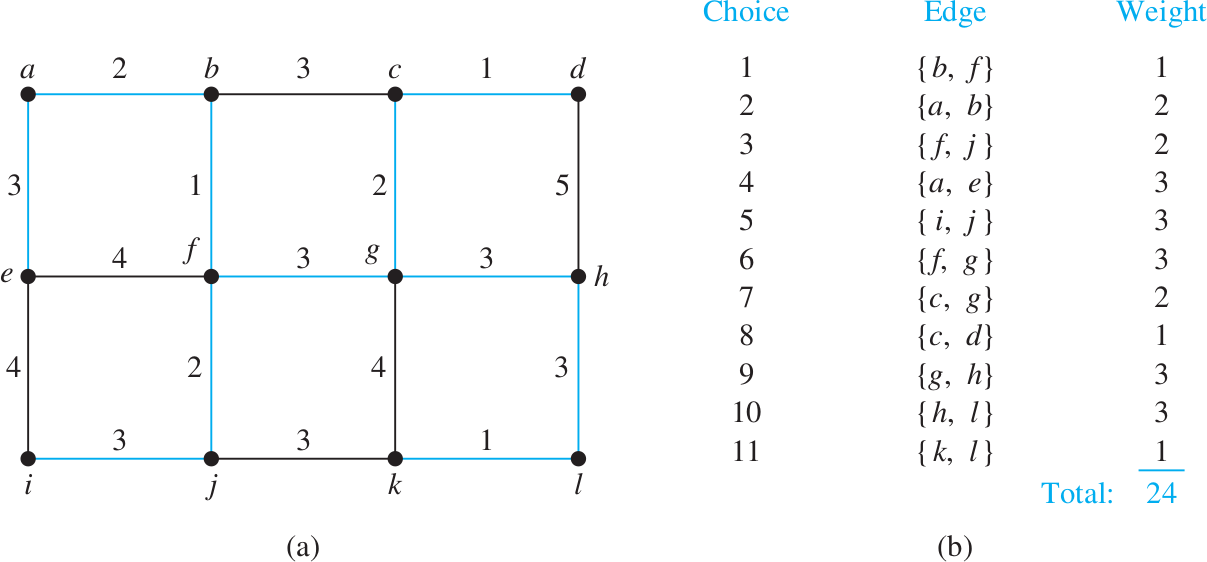
\includegraphics[width=\textwidth]{tree-spanning-prim}
\end{frame}

\begin{frame}{Reiknirit Kruskals}
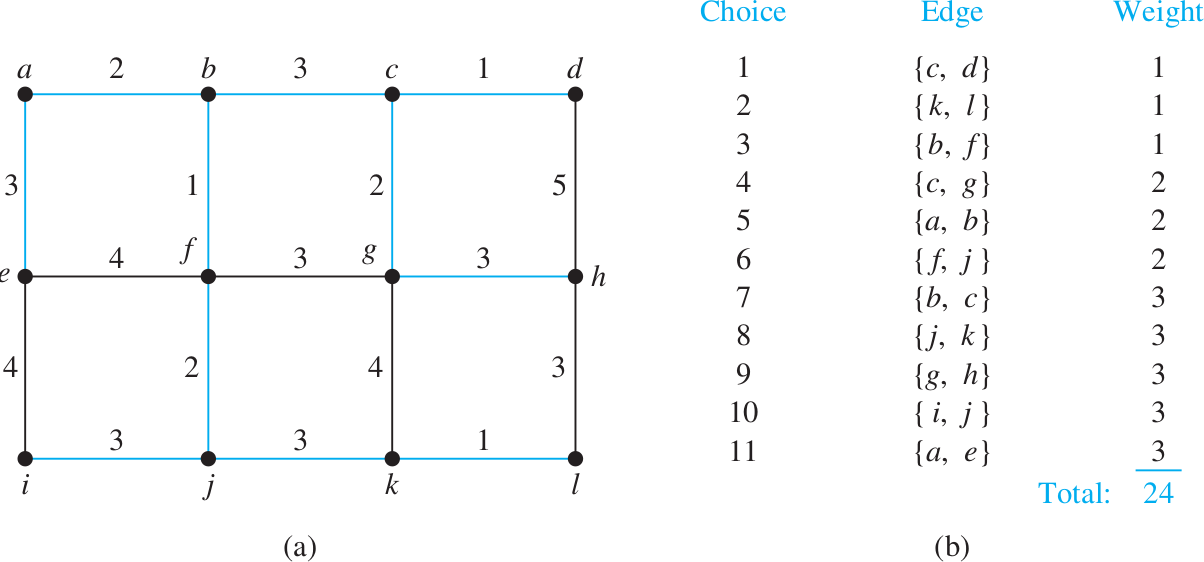
\includegraphics[width=\textwidth]{tree-spanning-kruskal}
\end{frame}


\section{Endanlegar stöðuvélar}

\begin{frame}{Endanlegar stöðuvélar}
\begin{itemize}
 \item Hægt er að lýsa ýmsum vélum og forritum með því að nota endanlega stöðuvél (e. \emph{finite-state machine})
 \item Grundvallaratriði í stöðuvélum er hugmyndin um að útreikningum eða aðgerðum megi lýsa með ástöndum (e. \emph{state}) og færslum þeirra á milli
 \item Dæmi: Læst hringhlið í skemmtigarði
\end{itemize}
\begin{center}
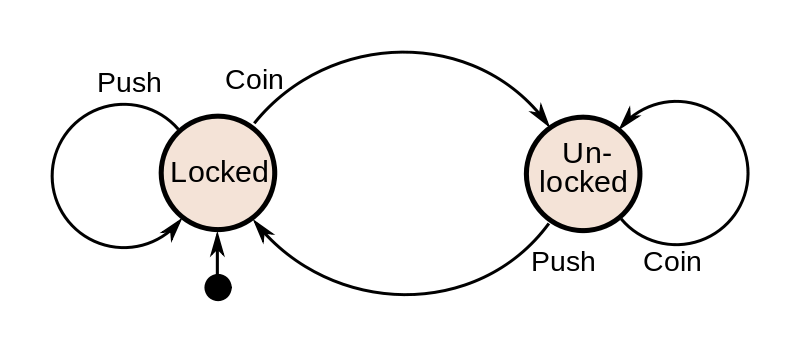
\includegraphics[width=0.5\textwidth]{turnstile-machine}
\end{center}
\end{frame}

\begin{frame}{Hagnýtingar}
\begin{itemize}
 \item Stöðuvélar og hugmyndir sem á þeim byggja koma mjög víða við
  \begin{itemize}
  \item Þýðendur og túlkar
  \item Reglulegar segðir
  \item Textagreining
  \item Tölvuleikir
 \end{itemize}
 \item Hjálpa til við að skipuleggja virkni forrita
 \item Notaðar í tölvunarfræði til formlegrar framsetningar á ``forritum''
\end{itemize}

\end{frame}


\section{Endanlegar stöðuvélar með úttaki}

\begin{frame}{Endanlegar stöðuvélar með úttaki}
Skoðum sérstaklega endanlegar stöðuvélar með úttaki.

\begin{tcolorbox}
Endanleg stöðuvél $M = (S, I, O, f, g, s_0 )$ samanstendur af
\begin{itemize}
 \item $S$, endanlegu mengi staða
 \item $I$, endanlegu inntaksstafrófi
 \item $O$, endanlegu úttaksstafrófi
 \item $f$, skiptifalli (e. \emph{transition function}) sem varpar hverju pari af stöðu og inntaki í nýja stöðu
 \item $g$, úttaksfalli (e. \emph{output function}) sem varpar hverju pari af stöðu og inntaki í eitt úttak
 \item $s_0$, upphafsstöðu
\end{itemize}

\end{tcolorbox}
\end{frame}

\begin{frame}{Dæmi}
Skoðum dæmi um stöðuvél. Myndin og taflan eru jafngild.
\begin{center}
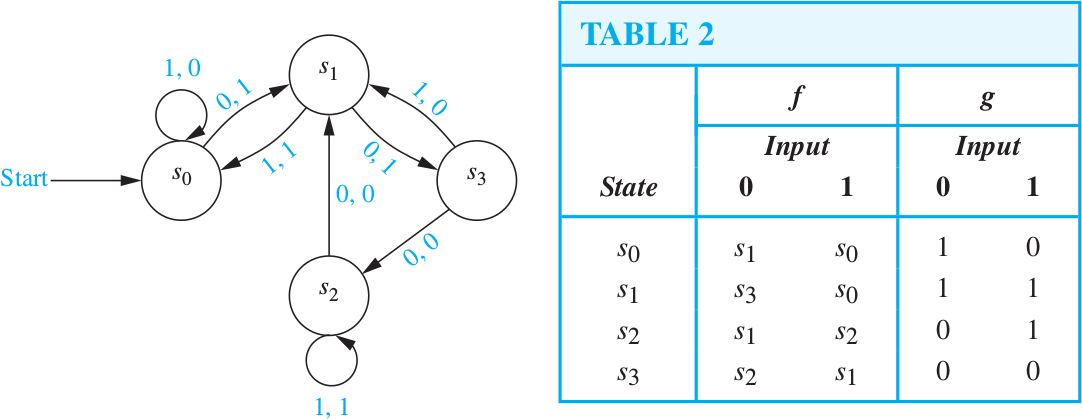
\includegraphics[width=0.9\textwidth]{fsm-example1}
\end{center}
Hvert er úttak stöðuvélarinnar þegar inntaksstrengurinn er $101011$? \pause Fáum $001000$.
\end{frame}

\begin{frame}{Dæmi}
\begin{columns}
\column{0.5\textwidth}
Skoðum stöðuvél sem seinkar inntaki sínu um einn bita.

\column{0.5\textwidth}
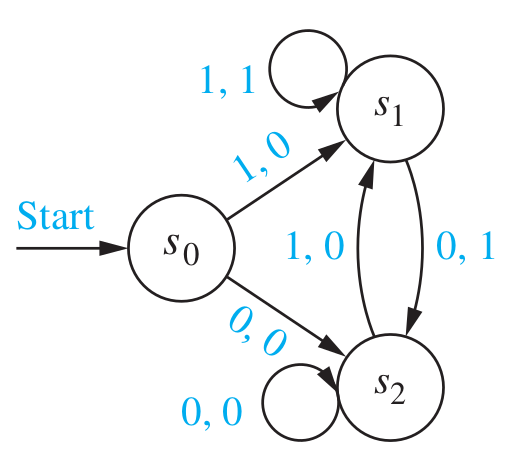
\includegraphics[width=\textwidth]{fsm-delay}
\end{columns}

\end{frame}

\begin{frame}{Dæmi}
\begin{columns}
\column{0.5\textwidth}
Skoðum stöðuvél sem leggur saman tvo bitastrengi. \pause

\column{0.5\textwidth}
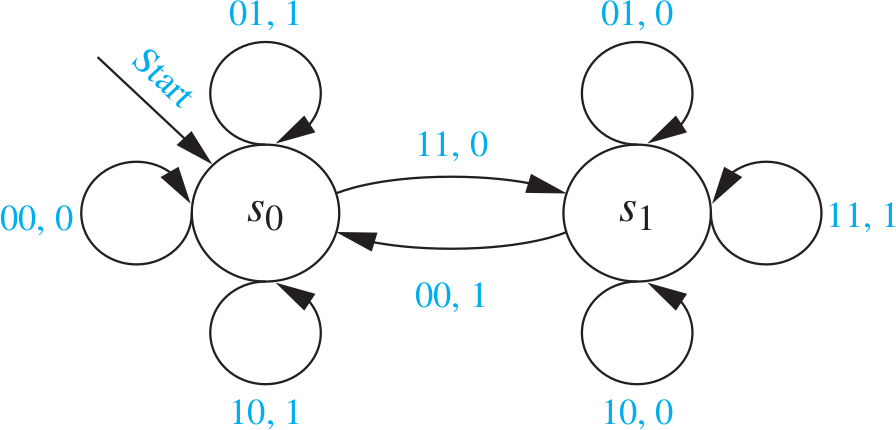
\includegraphics[width=\textwidth]{fsm-addition}
\end{columns}
\end{frame}

\begin{frame}{Sjálfsali}
\begin{itemize}
 \item Skoðum stöðuvél sem táknar sjálfsala
 \begin{itemize}
  \item Tekur við fimmköllum, tíköllum og 25-köllum
  \item Hafi upphæð a.m.k. 30 verið sett í vélina er hægt að ýta á appelsínugulan takka til að fá appelsínusafa eða rauðan takka til að fá eplasafa
  \item Hafi upphæð yfir 30 verið sett í vélina er afgangurinn samstundis gefinn til baka
  \item Möguleg úttök eru fjárhæðirnar $n$ (ekkert) 5, 10, 15, 20, 25, sem og appelsínusafi og eplasafi
 \end{itemize}
\end{itemize}
\end{frame}

\begin{frame}{Sjálfsali}
\begin{center}
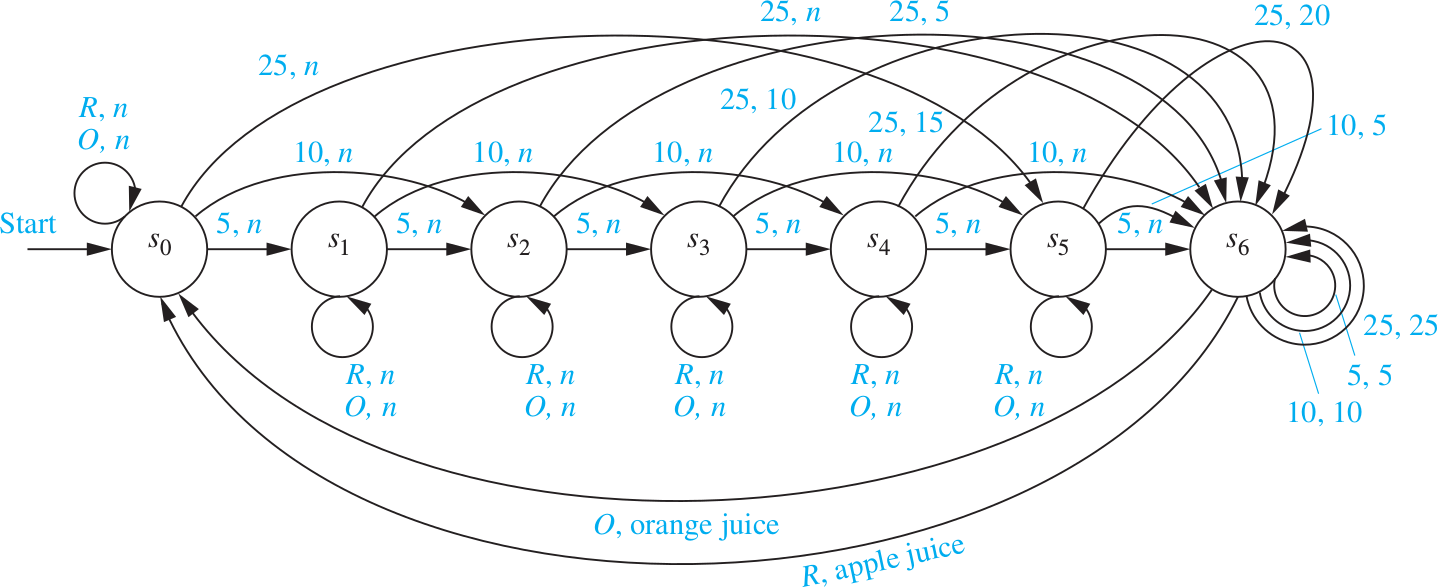
\includegraphics[width=\textwidth]{fsm-vending}
\end{center}
\end{frame}

\begin{frame}{Moore og Mealy}
\begin{itemize}
 \item Við höfum verið að skoða endanlegar stöðuvélar með úttaki þar sem úttakið kemur fram við færslu á milli staða
 \begin{itemize}
  \item Vélar af þessari gerð eru kallaðar Mealy-vélar
 \end{itemize}
 \item Annar möguleiki - endanlegar stöðuvélar með úttaki sem afmarkast eingöngu af stöðunum sjálfum
 \begin{itemize}
  \item Vélar af þessari gerð eru kallaðar Moore-vélar
  \item Skoðum þær ekki
 \end{itemize}
 \item Hvort tveggja er dæmi um ``transducer''
\end{itemize}
\end{frame}

\begin{frame}{Dæmi}
\begin{columns}
\column{0.5\textwidth}
Skoðum stöðuvél sem skilar 1 þá og því aðeins að sá hluti inntaksstrengsins sem hingað til hefur verið lesinn inn endi á $111$.

\column{0.5\textwidth}
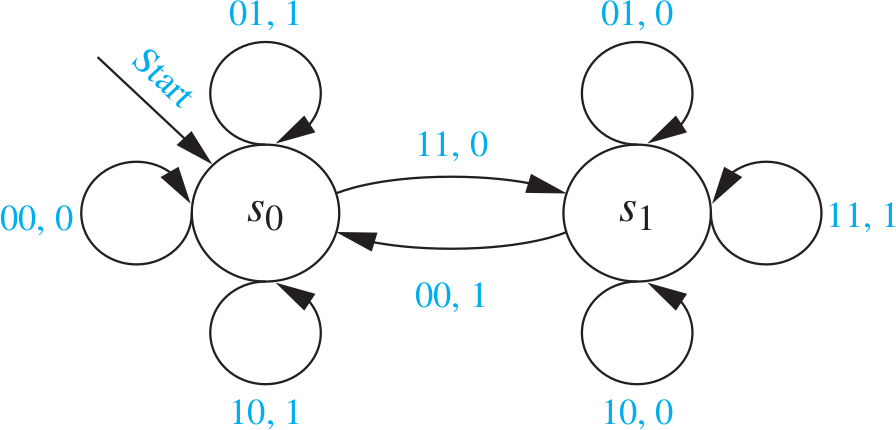
\includegraphics[width=\textwidth]{fsm-addition}
\end{columns}
\end{frame}

\section{Endanlegar stöðuvélar án úttaks}

\begin{frame}{Samþykkjarar}
Sumar stöðuvélar hafa ekki úttak, heldur eru þær notaðar til að samþykkja strengi eða hafna þeim. Köllum þær endanlega samþykkjara (e. \emph{acceptors}, í bók fjallað um sem \emph{finite-state automata}). 

\begin{center}
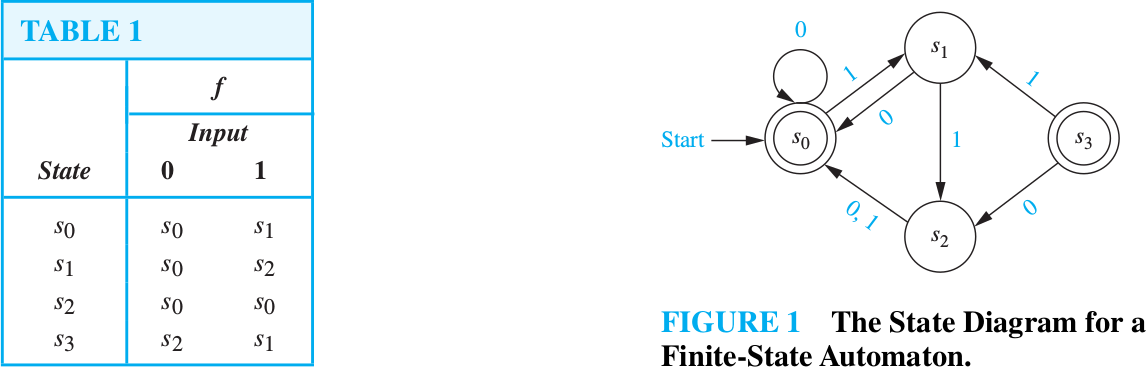
\includegraphics[width=\textwidth]{dfa-example1}
\end{center}


\end{frame}

\begin{frame}{Samþykkjarar}
\begin{tcolorbox}[title=Samþykkjarar]
Endanlegur samþykkjari $M = (S, I , f, s_0, F)$ samanstendur af:
\begin{itemize}
 \item $S$, endanlegu mengi staða
 \item $I$, endanlegu inntaksstafrófi
 \item $f$, skiptifalli sem varpar hverju pari af stöðu og inntaki í nýja stöðu
 \item $s_0$, upphafsstöðu
 \item $F$, hlutmengi í $S$ sem táknar lokastöður
\end{itemize}
\end{tcolorbox}
\end{frame}

\begin{frame}{Mál og samþykkjarar}
\begin{tcolorbox}
Strengur $x$ er samþykktur (e. \emph{accepted} eða \emph{recognized}) af samþykkjara $M$ taki hann $M$ úr upphafsstöðu yfir í lokastöðu.

Málið sem $M$ samþykkir (e. \emph{the language accepted by $M$}) er mengi allra strengja sem $M$ samþykkir.
\end{tcolorbox}
Tvær stöðuvélar eru sagðar jafngildar ef þær samþykkja sama mál.
\end{frame}

\begin{frame}{Dæmi}
Hvaða mál samþykkir þessi vél?

\begin{center}
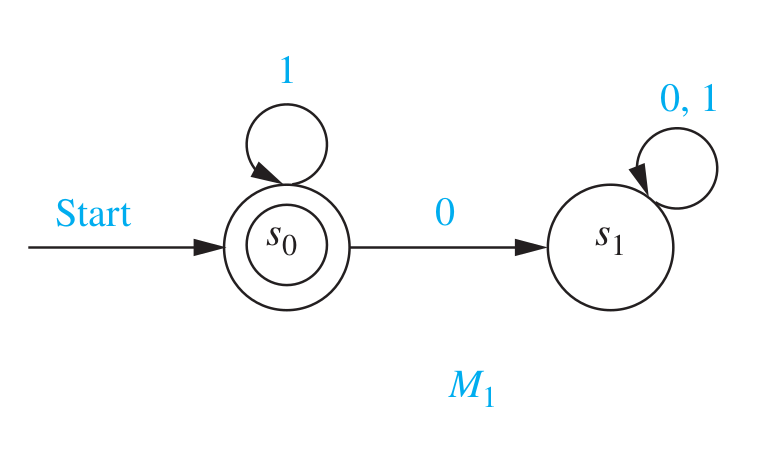
\includegraphics[width=0.6\textwidth]{dfa-example2}
\end{center}

\pause
Mál þeirra strengja sem eingöngu innihalda 0 eða fleiri ása.
\[
 L(M_1) = \{1^n | n \in 0, 1, 2, \ldots \}
\]

\end{frame}

\begin{frame}{Dæmi}
Hvaða mál samþykkir þessi vél?

\begin{center}
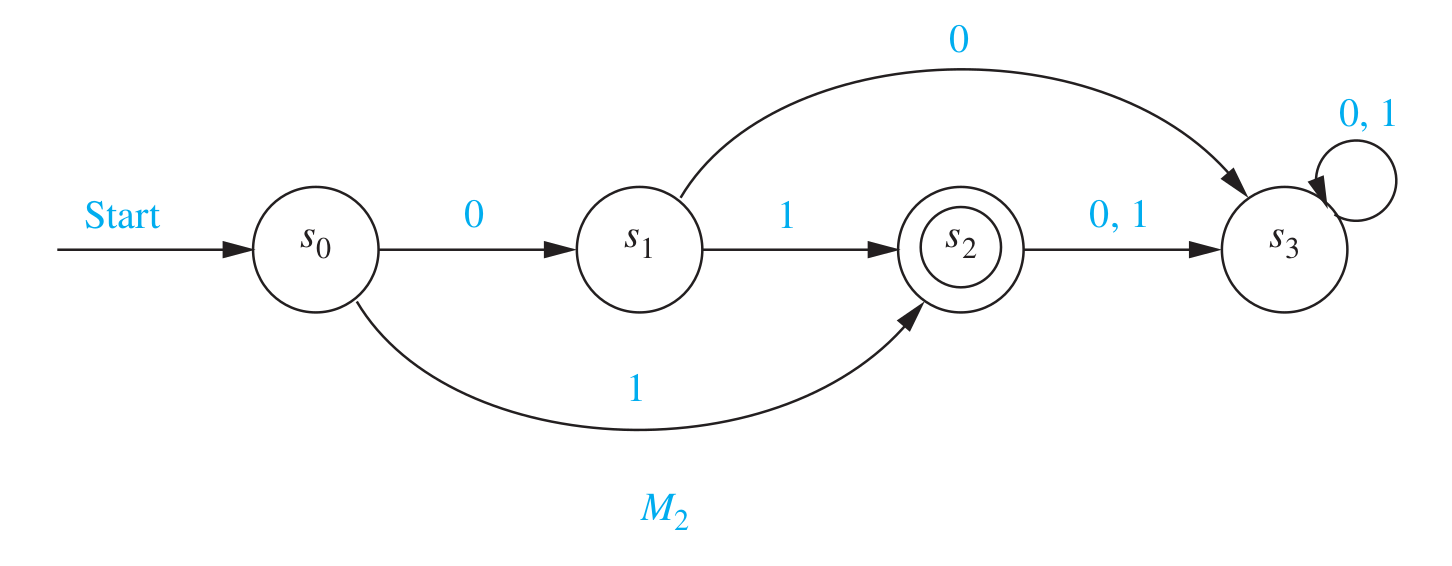
\includegraphics[width=\textwidth]{dfa-example3}
\end{center}

\pause
Við höfum nákvæmlega tvær leiðir til að komast í lokastöðu.
\[
 L(M_2) = \{1,01\}
\]

\end{frame}

\begin{frame}{Dæmi}
\begin{itemize}
 \item Getum við búið til stöðuvélar (samþykkjara) sem samþykkja eftirfarandi mál?
 \begin{itemize}
  \item Mengi bitastrengja sem byrja á 00
  \item Mengi bitastrengja sem innihalda 00
  \item Mengi bitastrengja sem innihalda ekki 00
 \end{itemize}
\end{itemize}
\end{frame}

\begin{frame}{Brigðgengni og löggengni}
\begin{itemize}
 \item Þeir samþykkjarar sem við höfum skoðað hér hafa varpað öllum mögulegum stöðu-inntaks pörum í nákvæmlega eina aðra stöðu
 \begin{itemize}
  \item Slíkar stöðuvélar eru kallaðar löggengar endanlegar stöðuvélar (e. \emph{deterministic})
 \end{itemize}
 \item Gætum líka skilgreint vélar þar sem hvert stöðu-inntakspar getur leitt okkur í meira en eina mismunandi stöðu
 \item Merkilegt - löggengar og brigðgengar endanlegar stöðuvélar eru jafn ``öflugar''
 \begin{itemize}
  \item Getum alltaf breytt brigðgengri vél í löggenga
 \end{itemize}
\end{itemize}
\end{frame}

\begin{frame}{Næst}
Turing-vélar
\end{frame}


\end{document}
